\documentclass[12pt]{article}
\usepackage{setspace, graphicx, fullpage, amssymb, amsmath, epsfig, natbib, array, multirow, hyperref}
\usepackage{amsfonts, bm} 
\usepackage{dcolumn}
\usepackage{subfigure, float} 
\usepackage[margin=.75in]{geometry} 
\usepackage{verbatim}
\usepackage{url}
\usepackage{enumerate}
\newcolumntype{d}[1]{D{.}{.}{#1}} 

\begin{document}
	
	\begin{center}
		Update: 16 November 2016
	\end{center}

I conducted a number of additional  In checking for the different responsiveness scores calculated, I found that in our Original Simulated Annealing, members were less responsive on party call votes than noncall votes 51.2\% of the time. In the flip flop vote sampling version this was the case 71.7\% of the time. It occurred 61.8\% of the time in the hybrid model.

I have updated the figures and tables as requested at the previous meeting. The graphs can be found on page 2 while the relevant tables are tables 7-9, beginning on page 9.

Additionally, I conducted multinomial logit analysis on the hybrid model and the flip flop reassignment model for the three most troublesome Congresses: Congress 102, 103, and 109. The results from these analyses are shown in tables 1-6, below, beginning on page 6. What I find is that for Congress 102 \& 103, bills featured in the CQ Almanac are most often gray, though in Congress 109 they are more likely to be noncalls than gray, with gray holding essentially equal likelihood with party call as the code. In the hybrid specification (which saw the worst performance for Congress 109), votes which were close tended slightly toward being coded as noncalls compared to grays and slightly more toward grays than calls. Finally, many procedural votes are clearly identified by both specifications as noncalls, but the rest have nearly equal likelihood of being identified as calls or being stuck as grays.

With each model discussed in this week's update, I replicated figure 2 from Minozzi \& Volden (2013). These can be found beginning on page 3 with the original simulated annealing, followed by the flip flop reassignment algorithm, and finishing with the hybrid model. To me it looks like the hybrid model performs this best, but we should discuss this.

At present, I am running the hybrid and simulated annealing algorithms with multiple set seeds to see if the hybrid has issues similar to those of the original simulated annealing. I began this Sunday and - underestimating the time it would take - set it to run across all Congresses all 4 times required to model this. Even after realizing this I held out hope that it would be finished by today, and not wanting to throw out data which could better test the results, have allowed it to continue running. 

I have further been working toward both getting the algorithm to orient party free ideal points such that Republicans are higher than Democrats and a record of ideal points is stored in the output similar to the record of p-values or t-values. I have unfortunately hit a snag in the latter which prevents me from gaging success in the former, but am confident I will have this sorted out in short order.

For the next week (or two if we don't touch base next week) I am prepared to run any model specification(s) that are preferred on the Senate. As things stand now, I am not convinced we have found a clear ``winner'' in any of the sorting methods but I am certainly open to your input on the matter. I am also open to tweaking any of the models which seem promising in order to attempt to better replicate prior results and/or further reduce gray votes. 



\begin{table}[b]
	\begin{center}
		\begin{tabular}{l c c }
			\hline
			& noncall & party call \\
			\hline
			(Intercept)      & $3.34^{***}$  & $-1.86$      \\
			& $(0.42)$      & $(1.08)$     \\
			Procedural       & $1.20^{***}$  & $-0.72$      \\
			& $(0.34)$      & $(0.40)$     \\
			CQ Votes    & $-0.93^{*}$   & $-0.74$      \\
			& $(0.41)$      & $(0.48)$     \\
			Close Votes & $1.89^{***}$  & $1.49^{***}$ \\
			& $(0.35)$      & $(0.43)$     \\
			Whip Final - G     & $-4.59^{***}$ & $1.20$       \\
			& $(0.44)$      & $(1.08)$     \\
			Whip Final - W     & $-3.12^{*}$   & $7.44^{***}$ \\
			& $(1.24)$      & $(1.46)$     \\
			\hline
			AIC              & 585.93        & 585.93       \\
			BIC              & 642.21        & 642.21       \\
			Log\ Likelihood  & -280.97       & -280.97      \\
			Deviance         & 561.93        & 561.93       \\
			Num.\ obs.       & 804           & 804          \\
			\hline
			\multicolumn{3}{l}{\scriptsize{$^{***}p<0.001$, $^{**}p<0.01$, $^*p<0.05$}}
		\end{tabular}
		\caption{Hybrid Model, Congress 102}
	\end{center}
\end{table}

\begin{table}
	\begin{center}
		\begin{tabular}{l c c }
			\hline
			& noncall & party call \\
			\hline
			(Intercept)      & $2.58^{***}$  & $-2.50^{*}$   \\
			& $(0.31)$      & $(1.05)$      \\
			Procedural       & $0.08$        & $-1.39^{***}$ \\
			& $(0.24)$      & $(0.26)$      \\
			CQ Votes    & $-0.35$       & $-0.29$       \\
			& $(0.43)$      & $(0.39)$      \\
			Close Votes & $0.99^{**}$   & $0.56$        \\
			& $(0.38)$      & $(0.35)$      \\
			Whip Final - G     & $-3.23^{***}$ & $2.55^{*}$    \\
			& $(0.34)$      & $(1.05)$      \\
			Whip Final - W     & $-4.86^{***}$ & $5.96^{***}$  \\
			& $(0.81)$      & $(1.08)$      \\
			\hline
			AIC              & 1099.36       & 1099.36       \\
			BIC              & 1158.08       & 1158.08       \\
			Log\ Likelihood  & -537.68       & -537.68       \\
			Deviance         & 1075.36       & 1075.36       \\
			Num.\ obs.       & 986           & 986           \\
			\hline
			\multicolumn{3}{l}{\scriptsize{$^{***}p<0.001$, $^{**}p<0.01$, $^*p<0.05$}}
		\end{tabular}
		\caption{Hybrid Model, Congress 103}
	\end{center}
\end{table}

\begin{table}
	\begin{center}
		\begin{tabular}{l c c }
			\hline
			& noncall & party call \\
			\hline
			(Intercept)      & $0.02$       & $-0.64^{***}$ \\
			& $(0.16)$     & $(0.19)$      \\
			Procedural       & $1.24^{***}$ & $0.03$        \\
			& $(0.25)$     & $(0.27)$      \\
			CQ Votes    & $0.20$       & $1.78^{***}$  \\
			& $(0.41)$     & $(0.37)$      \\
			Close Votes & $0.60$       & $-0.51$       \\
			& $(0.41)$     & $(0.37)$      \\
			Whip Final - G     & $-0.30$      & $0.17$        \\
			& $(0.22)$     & $(0.23)$      \\
			Whip Final - W     & $0.40$       & $1.81^{***}$  \\
			& $(0.30)$     & $(0.29)$      \\
			\hline
			AIC              & 1780.11      & 1780.11       \\
			BIC              & 1838.13      & 1838.13       \\
			Log\ Likelihood  & -878.06      & -878.06       \\
			Deviance         & 1756.11      & 1756.11       \\
			Num.\ obs.       & 930          & 930           \\
			\hline
			\multicolumn{3}{l}{\scriptsize{$^{***}p<0.001$, $^{**}p<0.01$, $^*p<0.05$}}
		\end{tabular}
		\caption{Hybrid Model, Congress 109}
	\end{center}
\end{table}

\begin{table}
	\begin{center}
		\begin{tabular}{l c c }
			\hline
			& noncall & party call \\
			\hline
			(Intercept)      & $6.08^{***}$  & $-11.26$     \\
			& $(1.05)$      & $(241.44)$   \\
			Procedural       & $1.28^{***}$  & $-0.97^{*}$  \\
			& $(0.36)$      & $(0.49)$     \\
			CQ Votes    & $-1.87^{***}$ & $-0.12$      \\
			& $(0.45)$      & $(0.61)$     \\
			Close Votes & $2.15^{***}$  & $1.95^{***}$ \\
			& $(0.38)$      & $(0.52)$     \\
			Whip Final - G     & $-6.11^{***}$ & $9.48$       \\
			& $(1.04)$      & $(241.44)$   \\
			Whip Final - W     & $-5.94^{***}$ & $15.27$      \\
			& $(1.29)$      & $(241.44)$   \\
			\hline
			AIC              & 507.04        & 507.04       \\
			BIC              & 563.31        & 563.31       \\
			Log\ Likelihood  & -241.52       & -241.52      \\
			Deviance         & 483.04        & 483.04       \\
			Num.\ obs.       & 804           & 804          \\
			\hline
			\multicolumn{3}{l}{\scriptsize{$^{***}p<0.001$, $^{**}p<0.01$, $^*p<0.05$}}
		\end{tabular}
		\caption{Flip Flop Reassignment, Congress 102}
		\label{table:coefficients}
	\end{center}
\end{table}

\begin{table}
	\begin{center}
		\begin{tabular}{l c c }
			\hline
			& noncall & party call \\
			\hline
			(Intercept)      & $5.47^{***}$  & $-2.46$       \\
			& $(1.05)$      & $(3.80)$      \\
			Procedural       & $0.04$        & $-1.16^{***}$ \\
			& $(0.24)$      & $(0.25)$      \\
			CQ Votes    & $-0.44$       & $-0.25$       \\
			& $(0.44)$      & $(0.37)$      \\
			Close Votes & $0.77^{*}$    & $0.63$        \\
			& $(0.38)$      & $(0.33)$      \\
			Whip Final - G     & $-5.66^{***}$ & $1.89$        \\
			& $(1.05)$      & $(3.80)$      \\
			Whip Final - W     & $-7.97^{***}$ & $4.83$        \\
			& $(1.20)$      & $(3.80)$      \\
			\hline
			AIC              & 1081.11       & 1081.11       \\
			BIC              & 1139.83       & 1139.83       \\
			Log\ Likelihood  & -528.56       & -528.56       \\
			Deviance         & 1057.11       & 1057.11       \\
			Num.\ obs.       & 986           & 986           \\
			\hline
			\multicolumn{3}{l}{\scriptsize{$^{***}p<0.001$, $^{**}p<0.01$, $^*p<0.05$}}
		\end{tabular}
		\caption{Flip Flop Reassignment, Congress 103}
	\end{center}
\end{table}

\begin{table}
	\begin{center}
		\begin{tabular}{l c c }
			\hline
			& noncall & party call \\
			\hline
			(Intercept)      & $0.84^{***}$ & $-0.21$      \\
			& $(0.18)$     & $(0.21)$     \\
			Procedural       & $1.03^{**}$  & $-0.15$      \\
			& $(0.32)$     & $(0.34)$     \\
			CQ Votes    & $-0.09$      & $1.57^{***}$ \\
			& $(0.45)$     & $(0.43)$     \\
			Close Votes & $1.01^{*}$   & $-0.29$      \\
			& $(0.47)$     & $(0.44)$     \\
			Whip Final - G     & $-0.31$      & $0.38$       \\
			& $(0.26)$     & $(0.28)$     \\
			Whip Final - W     & $0.72$       & $2.47^{***}$ \\
			& $(0.42)$     & $(0.42)$     \\
			\hline
			AIC              & 1607.41      & 1607.41      \\
			BIC              & 1665.43      & 1665.43      \\
			Log\ Likelihood  & -791.71      & -791.71      \\
			Deviance         & 1583.41      & 1583.41      \\
			Num.\ obs.       & 930          & 930          \\
			\hline
			\multicolumn{3}{l}{\scriptsize{$^{***}p<0.001$, $^{**}p<0.01$, $^*p<0.05$}}
		\end{tabular}
		\caption{Flip Flop Reassignment, Congress 109}
	\end{center}
\end{table}


\begin{center}
	
	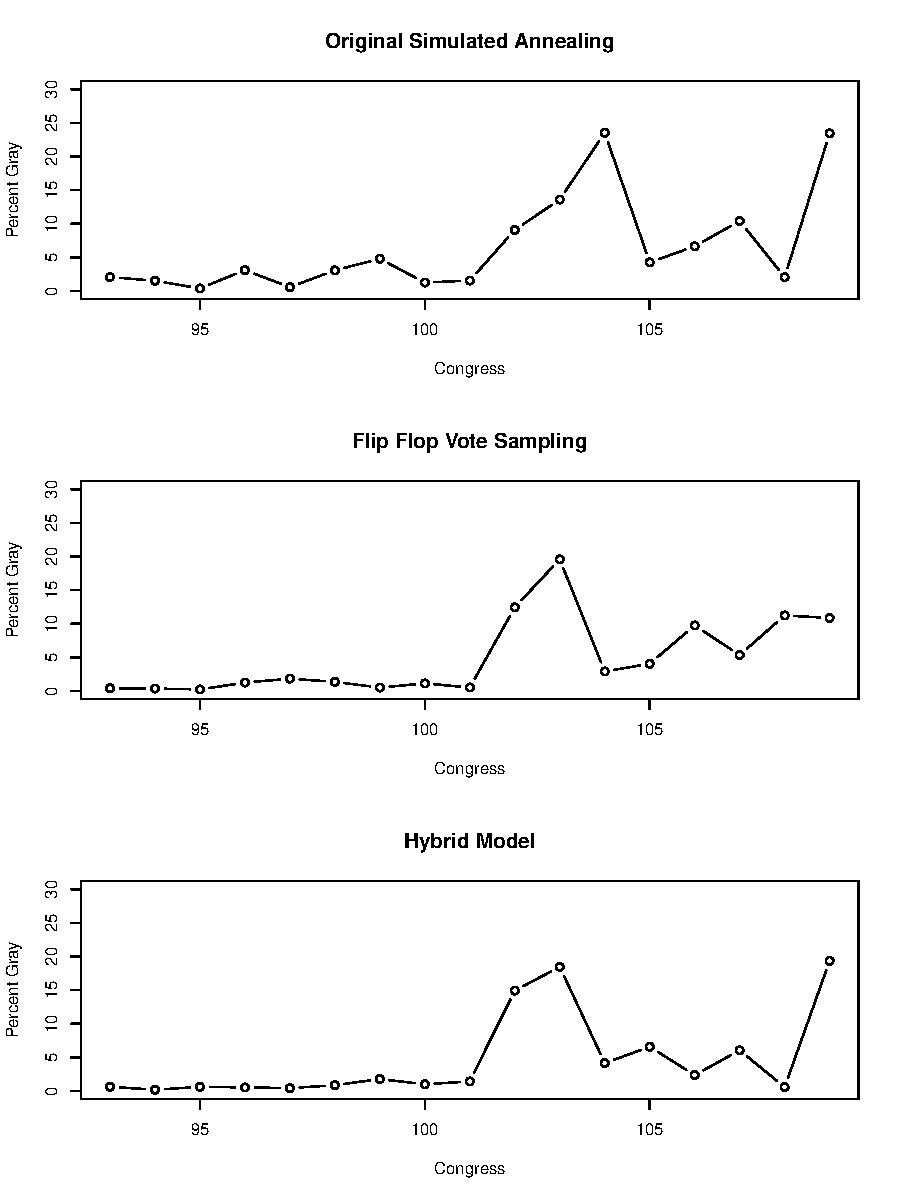
\includegraphics[]{C:/Users/Ethan/Documents/GitHub/partycalls/plots/gray_plot_nov16_1.pdf}
	
\end{center}

	
	\begin{table}[ht]
		\centering
		\caption{Original Simulated Annealing}
		\begin{tabular}{l c}
			\hline
			congress & \% Gray \\ 
			\hline
			93 & 2.1 \\ 
			94 & 1.5 \\ 
			95 & 0.4 \\ 
			96 & 3.1 \\ 
			97 & 0.6 \\ 
			98 & 3.1 \\ 
			99 & 4.8 \\ 
			100 & 1.3 \\ 
			101 & 1.5 \\ 
			102 & 9.1 \\ 
			103 & 13.6 \\ 
			104 & 23.5 \\ 
			105 & 4.3 \\ 
			106 & 6.6 \\ 
			107 & 10.4 \\ 
			108 & 2.0 \\ 
			109 & 23.4 \\ 
			\hline
			Mean: & 6.5 \\
			Median & 3.1 \\
			SD & 7.4 \\
			\hline
		\end{tabular}
	\end{table}
	


	\begin{table}[!htbp]
		\begin{center}
			\caption{Flip Flop Vote Sampling}
			\begin{tabular}[!hb]{lc}
				\hline
				Congress &  \% Gray  \\
				\hline
				
				93 & 0.4 \\ 
				94 & 0.4 \\ 
				95 & 0.2 \\ 
				96 & 1.2 \\ 
				97 & 1.8 \\ 
				98 & 1.4 \\ 
				99 & 0.5 \\ 
				100 & 1.1 \\ 
				101 & 0.5 \\ 
				102 & 12.4 \\ 
				103 & 19.6 \\ 
				104 & 2.9 \\ 
				105 & 4.0 \\ 
				106 & 9.7 \\ 
				107 & 5.3 \\ 
				108 & 11.2 \\ 
				109 & 10.9 \\ 
				\hline
				Mean & 4.9 \\
				Median & 1.8 \\
				SD & 5.7 \\
				\hline
			\end{tabular}
		\end{center}
	\end{table}
	


	\begin{table}[!htbp]
		\begin{center}
			\caption{Hybrid Model}
			\begin{tabular}[!hb]{lc}
				\hline
				Congress &  \% Gray  \\
				\hline
				93 & 0.6 \\ 
				94 & 0.2 \\ 
				95 & 0.6 \\ 
				96 & 0.5 \\ 
			    97 & 0.4 \\ 
				98 & 0.9 \\ 
				99 & 1.8 \\ 
				100 & 1.0 \\ 
				101 & 1.4 \\ 
				102 & 14.9 \\ 
				103 & 18.5 \\ 
				104 & 4.1 \\ 
				105 & 6.6 \\ 
				106 & 2.4 \\ 
				107 & 6.1 \\ 
				108 & 0.6 \\ 
				109 & 19.4 \\ 
				\hline
				Mean & 4.7 \\
				Median & 1.4 \\
				SD & 6.5 \\
				\hline
			\end{tabular}
		\end{center}
	\end{table}
	
	
	
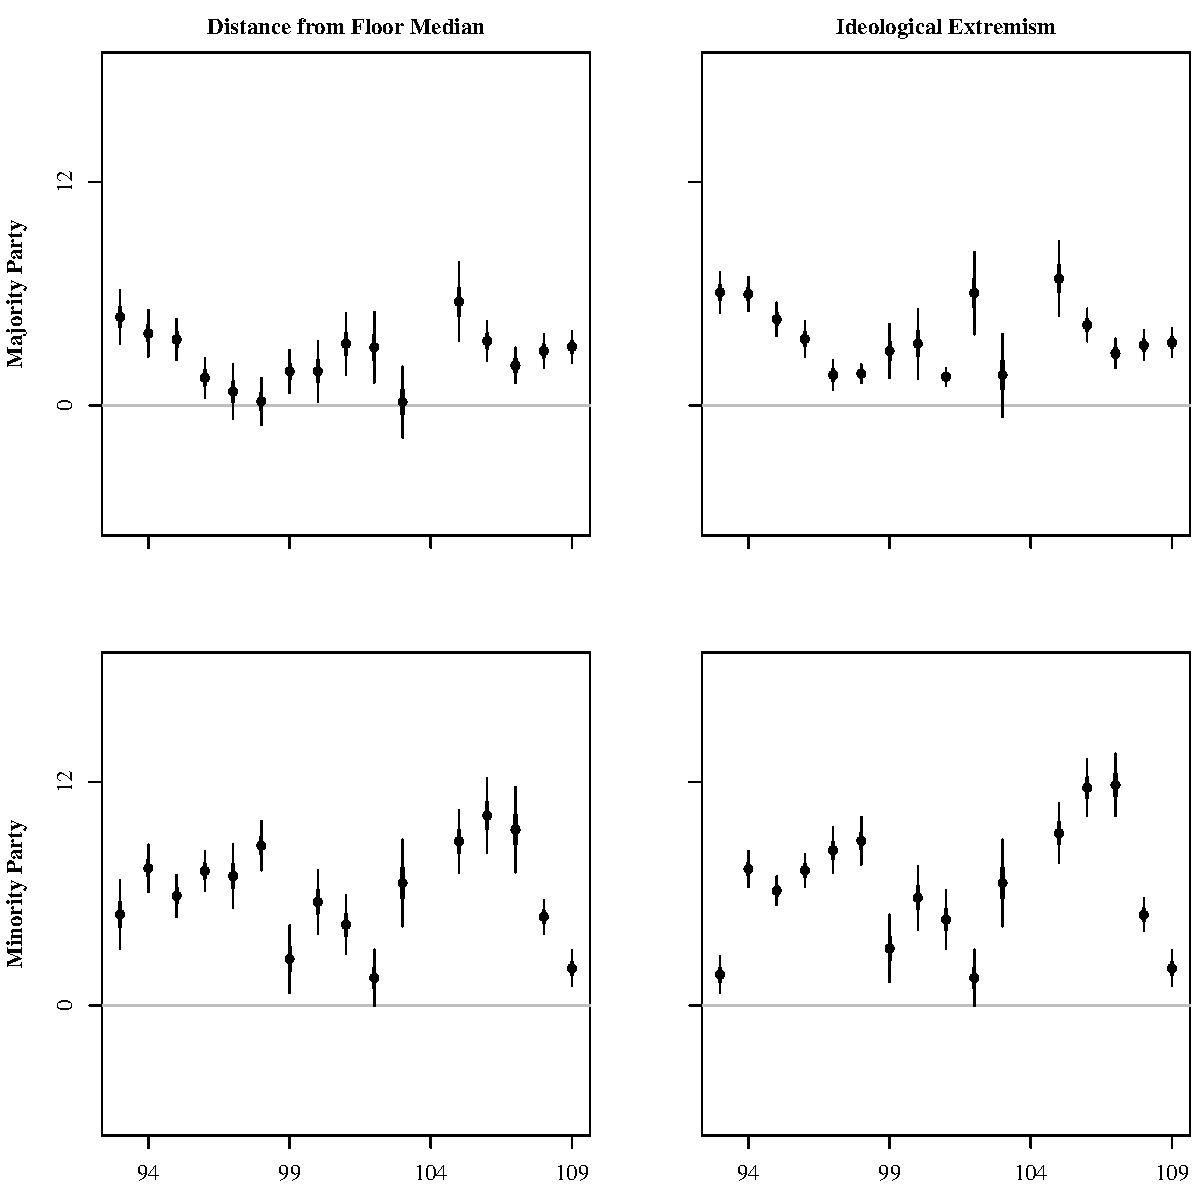
\includegraphics[width = \textwidth]{C:/Users/Ethan/Documents/GitHub/partycalls/plots/replicate-who-heeds-figure2_simannealing.pdf}
	
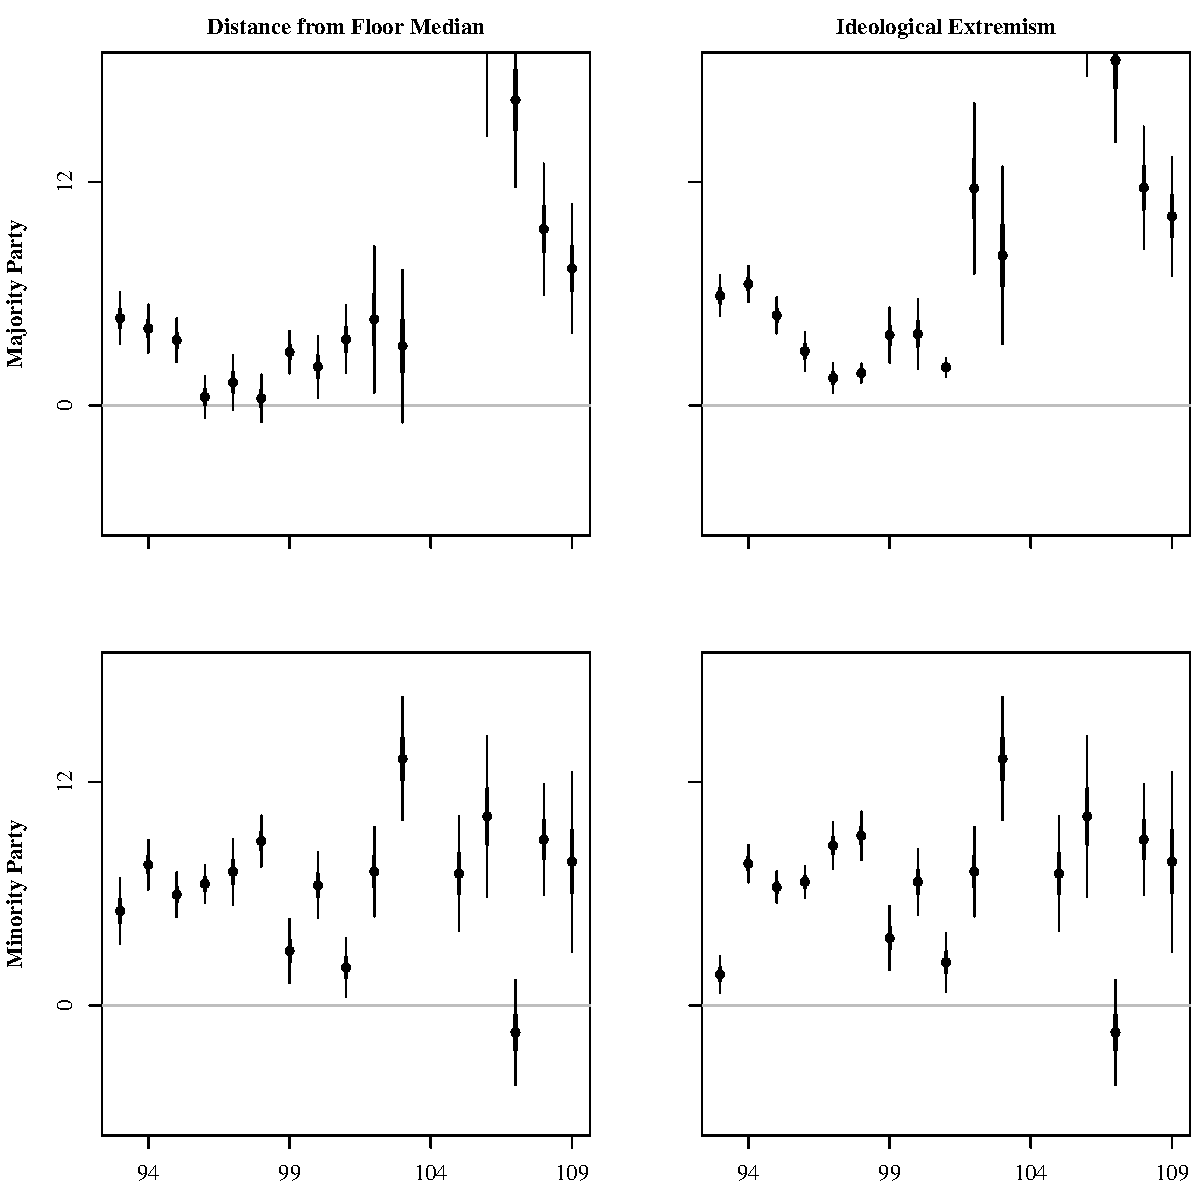
\includegraphics[width = \textwidth]{C:/Users/Ethan/Documents/GitHub/partycalls/plots/replicate-who-heeds-figure2_flipflop.pdf}
	
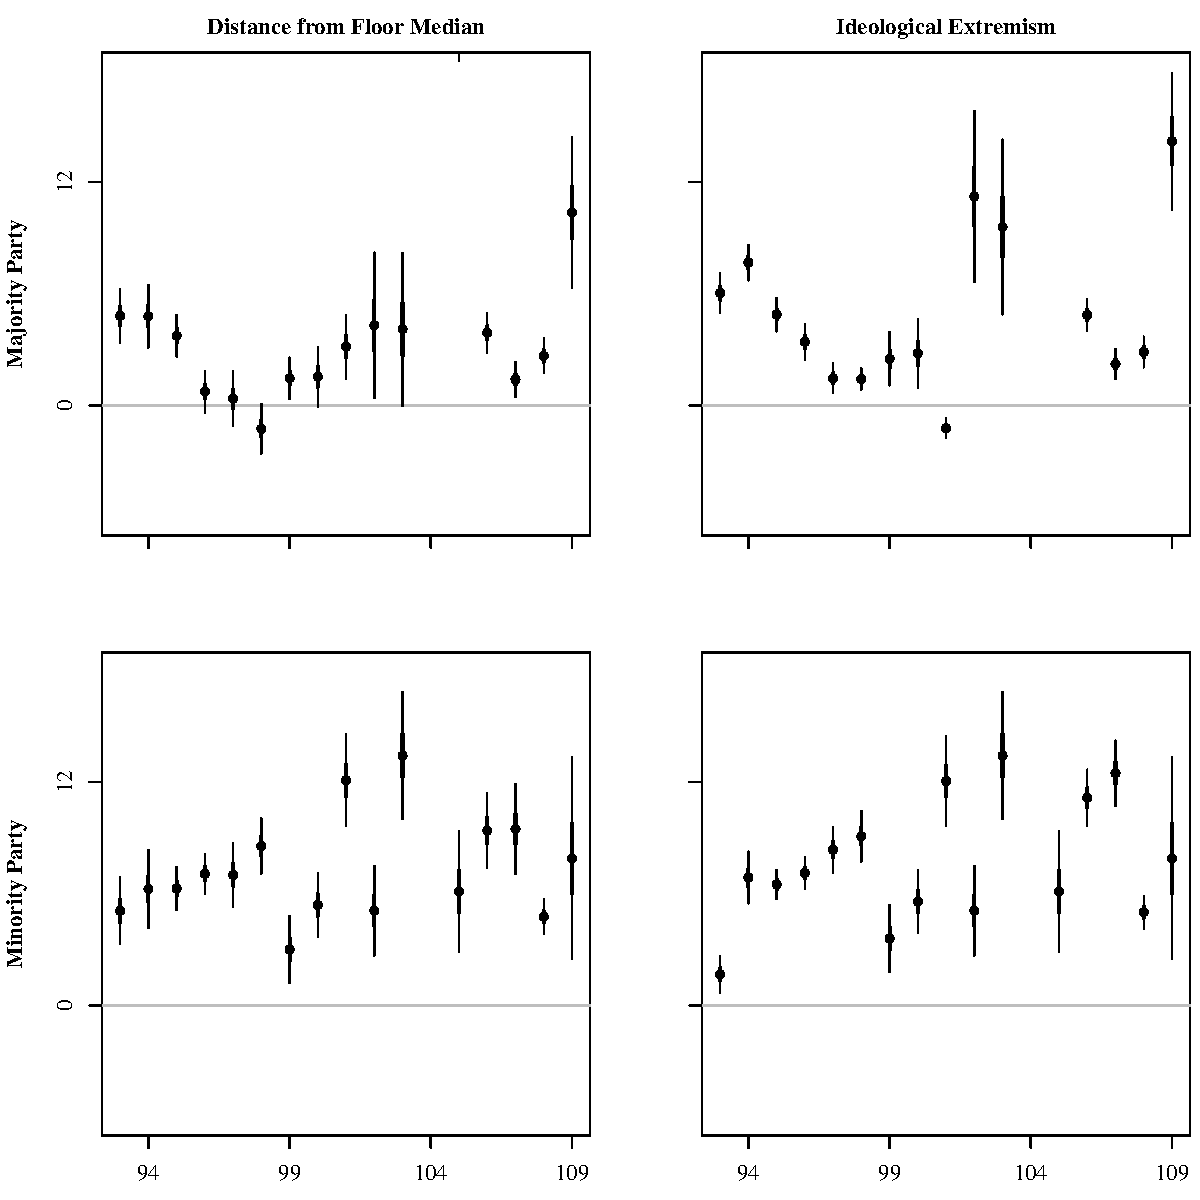
\includegraphics[width = \textwidth]{C:/Users/Ethan/Documents/GitHub/partycalls/plots/replicate-who-heeds-figure2_hybrid.pdf}
	
	
	
	
	
	
\end{document}